\documentclass{beamer}
\usetheme{default}
\usecolortheme{seahorse}
\usepackage[utf8]{inputenc}
\usepackage{graphicx}
\usepackage{booktabs}
\usepackage{amsmath}
\usepackage{natbib}
\usepackage[english]{babel}
\usepackage{hyphenat}
\usepackage{tikz}
\usetikzlibrary{shapes,arrows.meta,positioning}

\title[Lecture 3]{Reliability and Validity of a Measure}
\subtitle{Advanced Master in Agricultural Economics and Policy}
\author{Giovanbattista Califano}
\date[Portici, 24/04/2026]{Attitudinal Scales for the Study \\ of Consumer Preferences \\ April 24, 2026}
\institute[UNINA]{University of Naples Federico II, giovanbattista.califano@unina.it}

\AtBeginSection[]
{
  \begin{frame}<beamer>
    \frametitle{Moving on to...}
    \tableofcontents[currentsection]
  \end{frame}
}

\begin{document}

\frame{\titlepage}

\begin{frame}{Roadmap}
    \begin{center}
        \begin{tabular}{|l|l|c|}
        \hline
        20/04 &  Hello, Psychometrics! & $\checkmark$ \\
        \hline
        23/04 &  The Questionnaire & $\checkmark$ \\
        \hline
        24/04 & Reliability and Validity of a Measure & $\bigcirc$ \\
        \hline
        27/04 & Latent Variables: Reflective or Formative? & $\bigcirc$ \\
        \hline
        30/04 & A Bit of SEM & $\bigcirc$ \\
        \hline
        07/05 & Stata Stata Stata Stata Stata Stata Stata & $\bigcirc$ \\
        \hline
        \end{tabular}
    \end{center}
\vspace{0.1cm}
\footnotesize
Recommended readings: \\
\begin{itemize}
    \item Chapters 4 and 7 from \cite{jhangiani2019research}
    \item Chapters 7, 10 and 14 from \cite{olivero2022psicologia}
    \item Chapter 12 from \cite{mehmetoglu2022applied}
\end{itemize}
\scriptsize
\bibliographystyle{apalike}
\bibliography{text}
\end{frame}

\begin{frame}{Before we begin...}
\centering
    
\includegraphics[width=0.45\linewidth]{survey.png}
\end{frame}

\begin{frame}{Previously on...}
\begin{block}{What do we mean by measurement?}
    The \textit{systematic} assignment of a score to entities (individuals, objects, events...), such that the score represents a characteristic of those entities.
\end{block}
\pause
\begin{itemize}
    \item But how do we know that score \textbf{truly} represents the characteristic we want to study?
    \item Researchers do not take this for granted...
\end{itemize}
\end{frame}

\begin{frame}{Example}
\begin{block}{Califano's intelligence test}
    Califano's test was developed to measure intelligence quotient. According to the test, a person's IQ is given by the number of letters in their name ($n$) multiplied by 20: \\
    \[
    IQ = n \cdot 20
    \]
\end{block}
\pause
\begin{itemize}
    \item This test is more \textbf{reliable} than most existing tests for measuring IQ :)
    \pause
    \item It might be quite \textbf{invalid} :(
\end{itemize}
\end{frame}

\section{Reliability}
\begin{frame}{Reliability of a measure}
    \begin{block}{Reliability}
        refers to the degree of \textbf{consistency} of a measure. Psychometrics focuses, in particular, on three types of reliability:
    \end{block}
    \begin{enumerate}
        \item Over time (\textit{test-retest})
        \item Across researchers (\textit{inter-rater})
        \item Across items (\textit{internal})
    \end{enumerate}
\end{frame}

\begin{frame}{Reliability over time}
    \begin{block}{Test-Retest}
        If the measured construct is hypothesised to be consistent over time, the scores should be as well. Reliability over time consists in studying the correlation between two measurement distributions obtained by administering the same test twice to the same group of subjects after a given time interval.
    \end{block}
    \begin{block}{Example}
        If a person is very intelligent today, they should be so a week from now too...
    \end{block}
\end{frame}

\begin{frame}{Reliability across researchers}
    \begin{block}{Inter-Rater}
        If different researchers use the same system to assign scores, these scores should be positively correlated with one another.
    \end{block}
\end{frame}

\begin{frame}{Reliability across items}
    \begin{block}{Internal}
        Internal reliability is generally the most relevant when using self-report instruments, and refers to the consistency of respondents' answers to a multi-item measure.
    \end{block}
\end{frame}

\begin{frame}{Reliability across items}
  \begin{block}{Food Technology Neophobia Scale (Cox \& Evans, 2008)}
    The FTNS is a popular instrument for measuring neophobia towards food technologies and is based on the Likert scale.
  \end{block}
  \vspace{0.3cm}
  \small
  \begin{tabular}{l l}
    \textbf{FTNS 1:} & I don't need to eat food made using new technology \\
    & because the food I already eat is fine \\
    \textbf{FTNS 2:} & New food technologies are something I am \\
    & uncertain about \\
    \textbf{FTNS 3:} & New food products are not healthier than \\
    & traditional foods \\
    \textbf{(...)}
  \end{tabular}
  \vspace{0.2cm}
  \begin{center}
    \footnotesize
    \begin{tabular}{ccccc}
      \toprule
      \textit{Strongly} & \textit{Disagree} & \textit{Neither agree} & \textit{Agree} & \textit{Strongly} \\
      \textit{disagree} &  & \textit{nor disagree} &  & \textit{agree} \\
      \midrule
      $\bigcirc$ & $\bigcirc$ & $\bigcirc$ & $\bigcirc$ & $\bigcirc$ \\
      \bottomrule
    \end{tabular}
  \end{center}
\end{frame}

\tikzset{
  lv/.style = {draw=blue!80, fill=blue!10, very thick, ellipse, minimum height=1cm, minimum width=2cm, align=center}, mv/.style = {draw=blue!80, fill=blue!10, very thick, rectangle, minimum height=0.5cm, minimum width=1cm, align=center}, arrow/.style = {thick, ->, >=Stealth}
}

\begin{frame}{Reliability across items}
    \centering
    \begin{tikzpicture}[node distance=1cm, auto]
        \node[mv] (i1) {FTNS 1};
        \node[mv, below=of i1] (i2) {FTNS 2};
        \node[mv, below=of i2] (i3) {FTNS 3};
        \node[mv, below=of i3] (i4) {FTNS 4};
        \node[mv, below=of i4] (ik) {FTNS k};
        \node[lv, right=of i3] (FTN) {Food Technology \\ Neophobia};
        \draw[arrow] (FTN) -- (i1);
        \draw[arrow] (FTN) -- (i2);
        \draw[arrow] (FTN) -- (i3);
        \draw[arrow] (FTN) -- (i4);
        \draw[arrow] (FTN) -- (ik);
        \draw[loosely dotted, very thick] (i4) -- (ik);
    \end{tikzpicture}
\end{frame}

\begin{frame}{Reliability across items}
    The internal consistency of a scale can be measured in various ways, again based on the correlation index. \\
    \vspace{1em}
    The most intuitive approach is \textit{split-half} correlation:
    \begin{enumerate}
        \item The scale items are divided into two blocks (e.g. odd and even);
        \item Scores are aggregated for the two blocks, by sum or mean;
        \item The correlation index is calculated between the aggregated scores of the two blocks.
    \end{enumerate}
    \centering
    \vspace{1em}
    \textit{A split-half correlation coefficient $r > .80$ is generally considered an indicator of good internal consistency.}
\end{frame}

\begin{frame}{Reliability across items}
A more sophisticated and widely used approach is \textit{Cronbach's alpha}, defined as:
\[
\alpha = \frac{k}{k - 1} \left(1 - \frac{\sum_{i=1}^{k} \sigma^2_{Y_i}}{\sigma^2_X}\right)
\]
where:
\begin{itemize}
    \item \(k\) is the number of items composing the scale,
    \item \(\sigma^2_{Y_i}\) is the variance of item \(i\),
    \item \(\sigma^2_X\) is the variance of the total score (given by the sum of all items).
\end{itemize}
\vspace{1em}
\centering
\textit{In most cases, \(\alpha > .70\) is considered satisfactory.}
\end{frame}

\section{Validity}
\begin{frame}{Validity of a measure}
    We have seen how \textbf{Califano's test} for IQ might enjoy a good degree of \textit{reliability} (e.g. test-retest). What can we say about its \textit{validity}?
\end{frame}

\begin{frame}{Validity of a measure}
    Validity tells us how well the scores of a measure represent the characteristic they are supposed to represent. \\
    \vspace{1em}
    Validity is also divided into several types:
    \begin{itemize}
        \item Face validity
        \item Content validity
        \item Criterion validity
        \item Discriminant validity
    \end{itemize}
\end{frame}

\begin{frame}{Face and content validity}
    These are the two types of validity that are not established by quantitative methods. \textbf{Face validity} refers to common sense: it takes little to say that the number of letters in a name has nothing to do with intelligence. \\
    \vspace{1em}
    \textbf{Content validity}, on the other hand, refers to how well the measure \textit{covers} the construct of interest (e.g. the risk perception and perceived uselessness of new food technologies components in the FTNS).
\end{frame}

\begin{frame}{Criterion validity}
    A \textbf{criterion} can be any variable we think should be correlated with the construct we are trying to measure: \\
    \begin{itemize}
        \item Concurrent validity: when the criterion is measured at the same time as the construct;
        \item Predictive validity: when the criterion is measured after the construct;
        \item Convergent validity: when the criterion is an alternative measure of the same construct.
    \end{itemize}
\end{frame}

\begin{frame}{Discriminant validity}
    This is the degree to which the scores of a measure are \textit{not} correlated with measures of conceptually distinct variables.
\end{frame}

\begin{frame}{Criterion and discriminant validity}
    \small
    \begin{block}{An example}
    Suppose we want to test the criterion and discriminant validity of a scale measuring self-efficacy in tackling the master's programme.
        \begin{itemize}
            \item \textbf{Concurrent validity}: self-efficacy in tackling the master's should be positively correlated with attitudes towards Stata;
            \item \textbf{Predictive validity}: self-efficacy in tackling the master's should be able to predict the average grade obtained during the master's;
            \item \textbf{Convergent validity}: if we had another scale measuring the same self-efficacy, the two scales should show a positive correlation with each other;
            \item \textbf{Discriminant validity}: self-efficacy refers to confidence in one's ability to tackle specific tasks or situations, while self-esteem is a general evaluation of oneself. The two measures should therefore not be too highly correlated.
        \end{itemize}
    \end{block}
\end{frame}

\begin{frame}{Summary}
\centering
\begin{tabular}{ccc}
     Reliability & $\equiv$ & Precision \\
     Validity & $\equiv$ & Accuracy
\end{tabular}
\vspace{1em}
\begin{center}
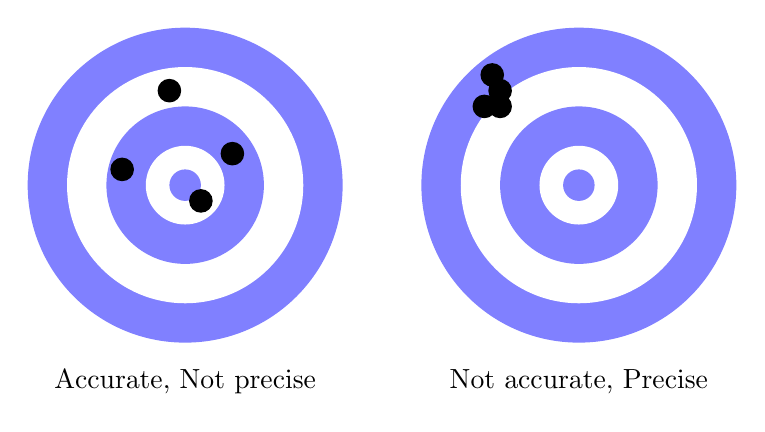
\begin{tikzpicture}
    % First target (High Accuracy, Low Precision)
    \begin{scope}
        \fill[blue!50] (0,0) circle (2);
        \fill[white] (0,0) circle (1.5);
        \fill[blue!50] (0,0) circle (1);
        \fill[white] (0,0) circle (0.5);
        \fill[blue!50] (0,0) circle (0.2);
        \fill (0.6,0.4) circle (0.15);
        \fill (-0.8,0.2) circle (0.15);
        \fill (0.2,-0.2) circle (0.15);
        \fill (-0.2,1.2) circle (0.15);
        \node at (0,-2.5) {Accurate, Not precise};
    \end{scope}
    \begin{scope}[xshift=5cm]
        \fill[blue!50] (0,0) circle (2);
        \fill[white] (0,0) circle (1.5);
        \fill[blue!50] (0,0) circle (1);
        \fill[white] (0,0) circle (0.5);
        \fill[blue!50] (0,0) circle (0.2);
        \fill (-1.2,1) circle (0.15);
        \fill (-1,1.2) circle (0.15);
        \fill (-1.1,1.4) circle (0.15);
        \fill (-1,1) circle (0.15);
        \node at (0,-2.5) {Not accurate, Precise};
    \end{scope}
\end{tikzpicture}
\end{center}
\end{frame}

\begin{frame}{Summary}
    \begin{itemize}
        \item Measuring a psychological construct requires four fundamental steps:
        \begin{enumerate}
            \item \textbf{Conceptual definition}: clarifying what is meant by the construct;
            \item \textbf{Operational definition}: translating the construct into something observable and measurable;
            \item \textbf{Implementation of the measure}: choosing or building the appropriate instrument;
            \item \textbf{Evaluation of the measure}: testing the instrument to verify its validity and reliability.
        \end{enumerate}
    \end{itemize}
\end{frame}

\begin{frame}{Summary}
    \textbf{1. Conceptual definition}
    \begin{itemize}
        \item A clear definition of the construct is needed.
        \item Consulting the scientific literature is essential.
    \end{itemize}
    \vspace{0.5em}
    \textbf{2. Operational definition}
    \begin{itemize}
        \item Specifies \emph{how} the construct will be measured.
        \item Multiple operational definitions of the same construct are possible.
    \end{itemize}
\end{frame}

\begin{frame}{Summary}
    \textbf{3. Implementing the measure}
    \begin{itemize}
        \item Using an existing instrument: faster, already validated, comparable with other studies.
        \item Creating a new measure: only if \emph{necessary}; pay attention to simplicity, clarity and number of items.
    \end{itemize}
    \vspace{0.5em}
    \textbf{4. Evaluating the measure}
    \begin{itemize}
        \item Preliminary testing with a few participants.
        \item Check: clarity of instructions, timing, comprehensibility.
        \item Collect feedback to correct any issues before data collection.
    \end{itemize}
\end{frame}

\section{Stata}
\begin{frame}{clear all ;)}
    \texttt{. webuse set https://califano.xyz/data} \\
    \texttt{. webuse masteristi}
\end{frame}

\end{document}
